\section{Управление в скользящих режимах}\label{sec:ch3/sec3}

\subsection{Теоретические основы многорежимного управления в скользящих режимах}\label{subsec:ch3/sec3/sub1}

Метод управления в скользящих режимах представляет собой робастный подход к управлению нелинейными системами,
основанный на переключении структуры управления для обеспечения движения изображающей точки системы вдоль заданной поверхности скольжения в
пространстве состояний. Данный метод особенно эффективен для систем с существенными нелинейностями и неопределенностями, что делает его
перспективным для применения в электропневматических приводах с дискретными распределителями.

Динамика электропневматического привода может быть представлена в виде нелинейной системы дифференциальных уравнений:
\begin{equation}
	\dot{\mathbf{x}} = \mathbf{f}(\mathbf{x}, t) + \mathbf{B}(\mathbf{x})\mathbf{u},
\end{equation}
где $\mathbf{x} \in \mathbb{R}^n$ -- вектор состояния системы, включающий положение и скорость штока пневмоцилиндра, а также давления в полостях;
$\mathbf{f}(\mathbf{x}, t)$ -- вектор-функция, описывающая естественную динамику системы;
$\mathbf{B}(\mathbf{x})$ -- матрица управления; $\mathbf{u} \in \mathbb{R}^m$ -- вектор управляющих воздействий, соответствующий состояниям дискретных распределителей.

Ключевым элементом метода является определение поверхности скольжения в пространстве состояний, геометрическая интерпретация которой представлена на рисунке~\ref{fig:phase_plane}:
\begin{equation}
	s(\mathbf{x}, t) = 0,
\end{equation}
где $s(\mathbf{x}, t)$ -- функция переключения.

\begin{figure}[ht]
	\centerfloat{
		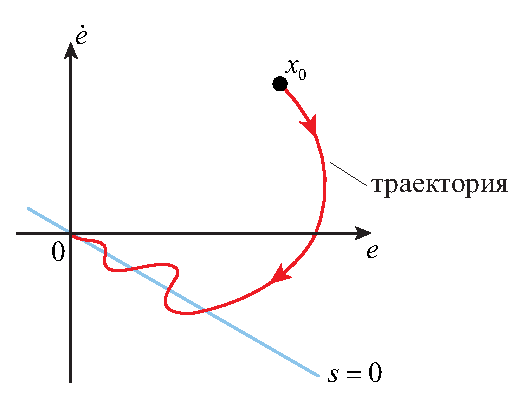
\includegraphics[]{part3/phase_plane.eps}
	}
	\caption{Геометрическая интерпретация поверхности скольжения в пространстве состояний}
	\label{fig:phase_plane}
\end{figure}

Для электропневматического привода с позиционным управлением целесообразно использовать функцию переключения вида:

\begin{equation}
	s(\mathbf{x}, t) = \dot{e} + \lambda e + \gamma\int_{0}^{t}e(\tau)d\tau,
\end{equation}
$\lambda, \gamma$ -- положительные константы, определяющие динамику системы в скольжении.

Как видно из рисунка~\ref{fig:phase_plane}, траектория системы стремится к поверхности скольжения под действием управления,
а затем движется вдоль неё к целевому состоянию. Области притяжения, показанные на рисунке,
обеспечивают сходимость траектории к поверхности скольжения с обеих сторон.

Существование скользящего режима обеспечивается выполнением условия притяжения к поверхности скольжения:
\begin{equation}
	s\dot{s} < 0.
\end{equation}

Данное условие может быть усилено введением требования η-притяжения:
\begin{equation}
	s\dot{s} \leq -\eta|s|,
\end{equation}
где $\eta$ -- положительная константа, определяющая скорость сходимости к поверхности скольжения.

В системах с дискретными распределителями управляющее воздействие формируется путем переключения между конечным набором состояний:
\begin{equation}
	\mathbf{u} \in {\mathbf{u}_1, \mathbf{u}_2, ..., \mathbf{u}_k},
\end{equation}
где $k$ -- количество допустимых комбинаций состояний распределителей. Закон управления принимает вид:

\begin{equation}
	\mathbf{u} = \begin{cases}
		\mathbf{u}^+, & s(\mathbf{x}, t) > \varepsilon      \\
		\mathbf{u}^0, & |s(\mathbf{x}, t)| \leq \varepsilon \\
		\mathbf{u}^-, & s(\mathbf{x}, t) < -\varepsilon
	\end{cases}
\end{equation}
где $\varepsilon$ -- ширина зоны гистерезиса, введенная для предотвращения высокочастотных переключений;
$\mathbf{u}^+, \mathbf{u}^0, \mathbf{u}^-$ -- векторы состояний распределителей.

Устойчивость системы может быть исследована с помощью функции Ляпунова:
\begin{equation}
	V = \frac{1}{2}s^2.
\end{equation}

Условие устойчивости требует:
\begin{equation}
	\dot{V} = s\dot{s} < 0.
\end{equation}

Характерной проблемой систем со скользящим управлением является возникновение высокочастотных колебаний
(chattering). Для их подавления применяется введение граничного слоя с непрерывной аппроксимацией разрывного управления:
\begin{equation}
	\mathbf{u} = \mathbf{u}^0 - \mathbf{K}\text{sat}\left(\frac{s}{\Phi}\right),
\end{equation}
где $\Phi$ -- ширина граничного слоя; $\text{sat}(\cdot)$ -- функция насыщения.

Динамическая адаптация ширины зоны гистерезиса может быть реализована согласно выражению:
\begin{equation}
	\varepsilon(t) = \varepsilon_0 + \beta\exp\left(-\alpha\left|\frac{ds}{dt}\right|\right),
\end{equation}
где $\varepsilon_0$ -- минимальная ширина зоны; $\alpha, \beta$ -- параметры адаптации.

Важным преимуществом скользящего управления является его робастность к
параметрическим возмущениям. При наличии неопределенностей в модели системы:
\begin{equation}
	\mathbf{f}(\mathbf{x}, t) = \mathbf{f}_0(\mathbf{x}, t) + \Delta\mathbf{f}(\mathbf{x}, t),
\end{equation}
где $\mathbf{f}_0(\mathbf{x}, t)$ -- номинальная модель;
$\Delta\mathbf{f}(\mathbf{x}, t)$ -- ограниченная неопределенность:

\begin{equation}
	|\Delta\mathbf{f}(\mathbf{x}, t)| \leq F_m(\mathbf{x}, t)
\end{equation}

При соответствующем выборе параметров управления система сохраняет устойчивость и обеспечивает требуемое качество управления.

\subsection{Многорежимное управление в скользящих режимах}\label{subsec:ch3/sec3/sub2}

Анализ динамики электропневматического привода с дискретными распределителями требует
систематического исследования поведения системы при различных конфигурациях поверхностей
скольжения. Рассмотрим математическое описание и особенности формирования управляющих
воздействий для каждой конфигурации, основываясь на результатах анализа режимов, представленных в разделе \ref{sec:ch3/sec1}.

В случае трехрежимного управления закон переключения может быть представлен в следующем виде:
\begin{equation}
	\mathbf{u}(s) = \begin{cases}
		[1,0,0,1], & s > \varepsilon      \\
		[0,0,0,0], & |s| \leq \varepsilon \\
		[0,1,1,0], & s < -\varepsilon
	\end{cases}
\end{equation}
где $\varepsilon$ -- параметр, определяющий ширину зоны переключения, $s$ - функция переключения, определяемая как:

Для данного случая функция переключения имеет вид:
\begin{equation}
	s = \dot{e} + \lambda e
\end{equation}
где $\lambda$ -- положительный коэффициент.

В фазовом пространстве векторное поле системы разделяется на три области линией
переключения $s = 0$. На рисунке \ref{fig:vector_field_linear} представлено
распределение векторного поля, где в области $s > \varepsilon$ векторы
скоростей направлены к линии переключения под действием
управления $\mathbf{u} = [1,0,0,1]$, соответствующего максимальному ускорению в положительном
направлении. При $s < -\varepsilon$ управление $\mathbf{u} = [0,1,1,0]$ формирует
векторное поле, обеспечивающее движение к линии переключения с противоположной
стороны. В зоне $|s| \leq \varepsilon$ все распределители закрыты $\mathbf{u} = [0,0,0,0]$,
что приводит к замедлению движения за счет сил трения и пневматической жесткости.
\begin{figure}[h]
	\centering
	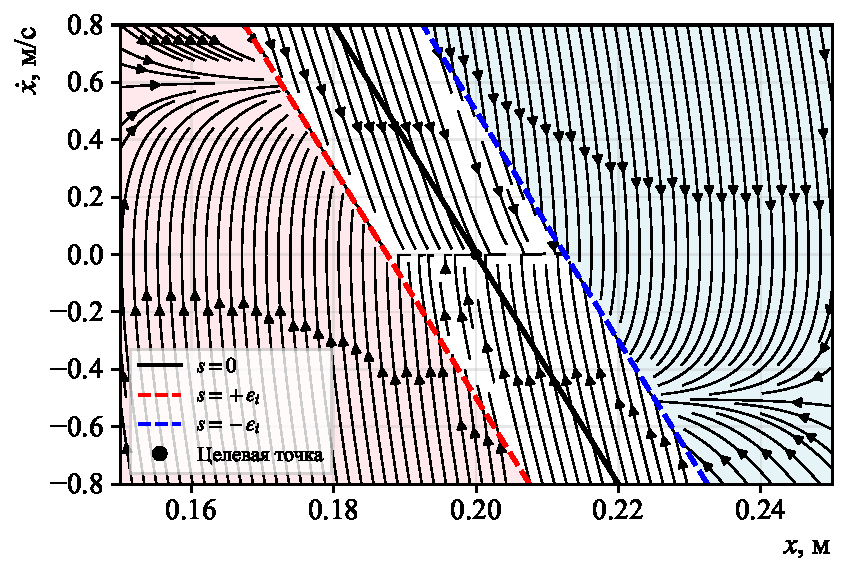
\includegraphics[]{part3/phase_portrait_3mode.pdf}
	\caption{Распределение векторного поля в фазовом пространстве для линейной поверхности первого порядка}
	\label{fig:vector_field_linear}
\end{figure}

При малых значениях параметра $\varepsilon$ возникает эффект <<дребезга>> (chattering),
обусловленный конечным быстродействием электромагнитных распределителей,
инерционностью термодинамических процессов и задержками в системе управления.
Математически эффект <<дребезга>> проявляется в высокочастотных осцилляциях функции
переключения, что может быть выражено соотношением:

\begin{equation}
	\lim_{t \to \infty} \frac{1}{T}\int_t^{t+T} |s(\tau)| d\tau > 0,
\end{equation}
где $T$ - период осцилляций.

На рисунке \ref{fig:ch3:transient_comparison_linear_mode3} представлены результаты моделирования
для двух значений границы коридора: $\varepsilon = 0,2$ и $\varepsilon = 0,01$.

\begin{figure}[h]
	\centering
	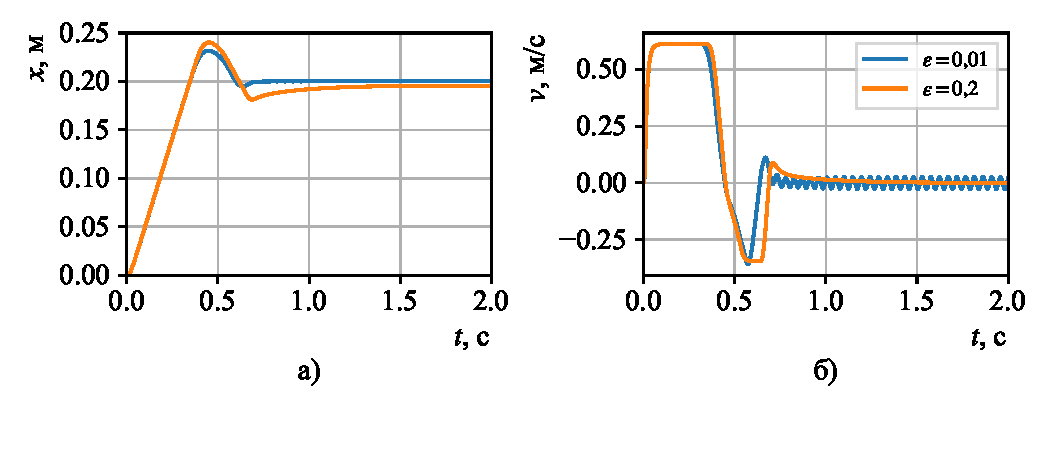
\includegraphics[]{part3/sliding_mode_linear_transients.pdf}
	\caption{Переходные процессы для 3 режимов управления с линейной поверхностью первого порядка}
	\label{fig:ch3:transient_comparison_linear_mode3}
\end{figure}

Увеличение параметра $\varepsilon$ позволяет стабилизировать процесс, однако приводит к
росту статической ошибки позиционирования, ограниченной соотношением:

\begin{equation}
	|e_{ss}| \leq \frac{\varepsilon}{\lambda}
\end{equation}

Для преодоления указанных ограничений предлагается использование многорежимного управления
с пятью или семью режимами, обеспечивающего более гибкое управление торможением
перед достижением целевого положения. При пятирежимном управлении закон управления имеет вид:

\begin{equation}\label{eq:control_law_5_mode}
	\mathbf{u}(s) = \begin{cases}
		[1,0,0,1], & s > \varepsilon_2                      \\
		[1,0,0,0], & \varepsilon_1 < s \leq \varepsilon_2   \\
		[0,0,0,0], & |s| \leq \varepsilon_1                 \\
		[0,0,1,0], & -\varepsilon_2 < s \leq -\varepsilon_1 \\
		[0,1,1,0], & s \leq -\varepsilon_2
	\end{cases}
\end{equation}
где $\varepsilon_1$, $\varepsilon_2$ -- параметры, определяющие границы зон переключения режимов ($\varepsilon_1 < \varepsilon_2$).

Дальнейшее развитие подхода привело к формированию семирежимного управления с более тонкой градацией торможения:

\begin{equation}\label{eq:control_law_7_mode}
	\mathbf{u}(s) = \begin{cases}
		[1,0,0,1], & s > \varepsilon_3                      \\
		[1,0,0,0], & \varepsilon_2 < s \leq \varepsilon_3   \\
		[0,0,0,1], & \varepsilon_1 < s \leq \varepsilon_2   \\
		[0,0,0,0], & |s| \leq \varepsilon_1                 \\
		[0,1,0,0], & -\varepsilon_2 < s \leq -\varepsilon_1 \\
		[0,0,1,0], & -\varepsilon_3 < s \leq -\varepsilon_2 \\
		[0,1,1,0], & s \leq -\varepsilon_3
	\end{cases}
\end{equation}
где $\varepsilon_1$, $\varepsilon_2$, $\varepsilon_3$ -- параметры, определяющие границы зон переключения режимов ($\varepsilon_1 < \varepsilon_2 < \varepsilon_3$).

Данные модификации обеспечивают более плавное снижение скорости движения перед включением режима удержания,
существенное уменьшение количества переключений распределителей и повышение точности позиционирования
без увеличения частоты переключений. При этом семирежимное управление позволяет достичь
наиболее точного позиционирования за счет более тонкой градации тормозных режимов.

На рисунах \ref{fig:vector_field_linear_5mode} и \ref{fig:vector_field_linear_7mode} представлены векторные поля
в фазовом пространстве для пятирежимного и семирежимного управления соответственно.

\begin{figure}[htbp]
	\centering
	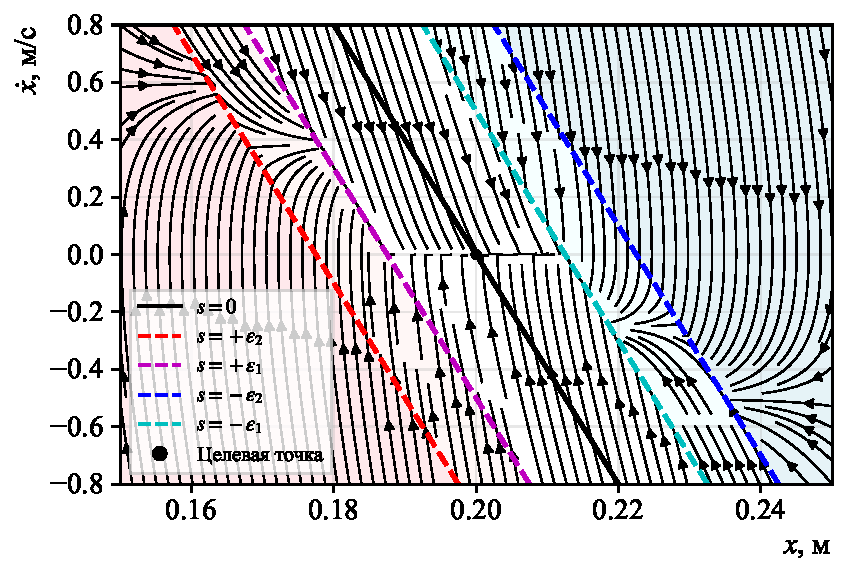
\includegraphics[]{part3/phase_portrait_5mode.pdf}
	\caption{Распределение векторного поля в фазовом пространстве для линейной поверхности первого порядка и пятирежимного управления}
	\label{fig:vector_field_linear_5mode}
\end{figure}

\begin{figure}[htbp]
	\centering
	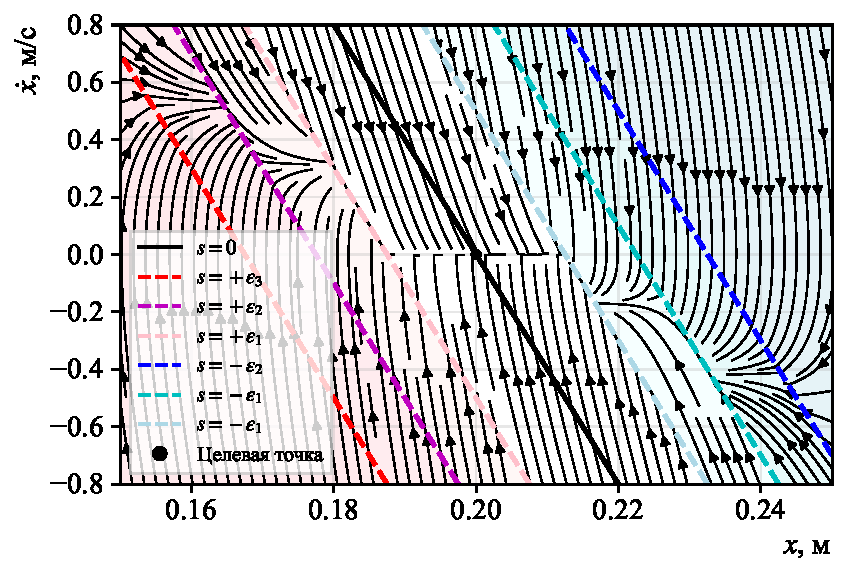
\includegraphics[]{part3/phase_portrait_7mode.pdf}
	\caption{Распределение векторного поля в фазовом пространстве для линейной поверхности первого порядка и семирежимного управления}
	\label{fig:vector_field_linear_7mode}
\end{figure}

\subsection{Анализ поверхностей скольжения}\label{subsec:ch3/sec3/sub3}

Исследование характера движения системы в фазовом пространстве требует детального рассмотрения математической
структуры и особенностей различных поверхностей скольжения.
Проанализируем три типа поверхностей: линейную, интегральную и терминальную при трехрежином управлении.

Линейная поверхность скольжения описывается выражением:

\begin{equation}
	s_1 = \dot{e} + \lambda_1 e,
\end{equation}
где $\lambda_1$ -- положительный коэффициент, определяющий наклон линии переключения в
фазовой плоскости.

Динамика системы в скользящем режиме описывается дифференциальным уравнением первого порядка:
\begin{equation}
	\dot{e} + \lambda_1 e = 0,
\end{equation}
обеспечивающим экспоненциальную сходимость ошибки к нулю с постоянной
времени $T = 1/\lambda_1$. Особенность данной поверхности заключается в
линейном характере убывания ошибки, что приводит к
относительно медленной сходимости при малых отклонениях от целевого положения.

На рисунке \ref{fig:smc_linear_wide} представлены результаты моделирования для линейной поверхности первого порядка при широком коридоре
($\varepsilon = \num{0.2}$) и значении коэффициента $\lambda_1 = 5$.

\begin{figure}[ht]
	\centering
	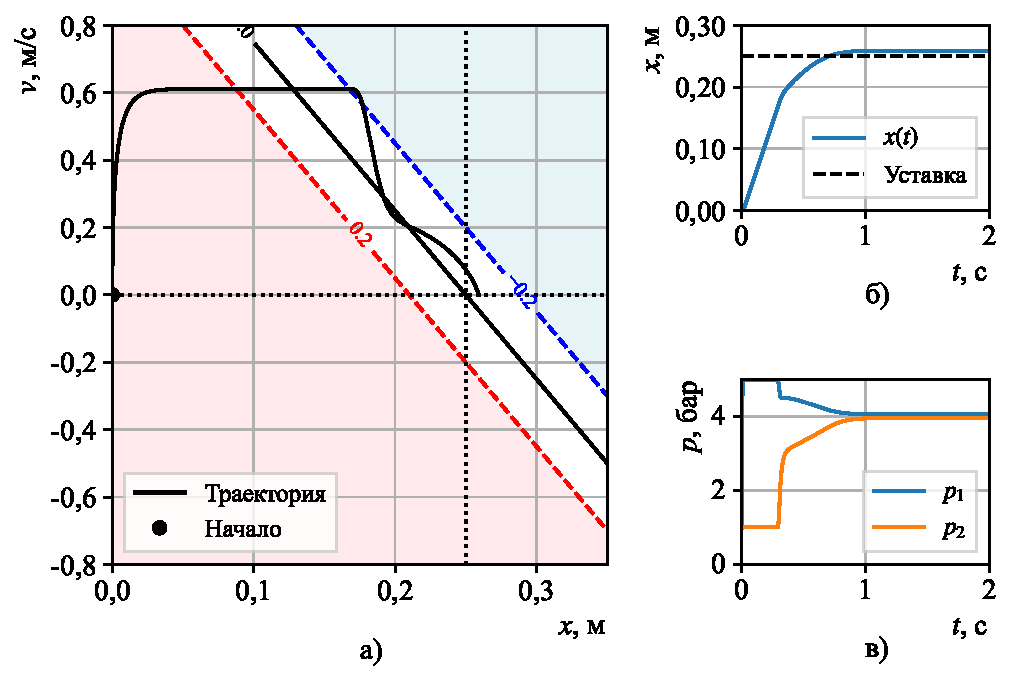
\includegraphics[]{part3/smc_linear_wide.pdf}
	\caption{Динамика системы в скользящем режиме с линейной поверхностью первого порядка при $\lambda_1 = \num{5}$~и~$\varepsilon=\num{0.2}$: \\
		а) фазовый портрет; б) переходной процесс; в) изменение давлений в полостях}
	\label{fig:smc_linear_wide}
\end{figure}

А при том же значении $\lambda$, но узком коридоре ($\varepsilon = \num{0.02}$) на рисунке \ref{fig:smc_linear_narrow}.

\begin{figure}[ht]
	\centering
	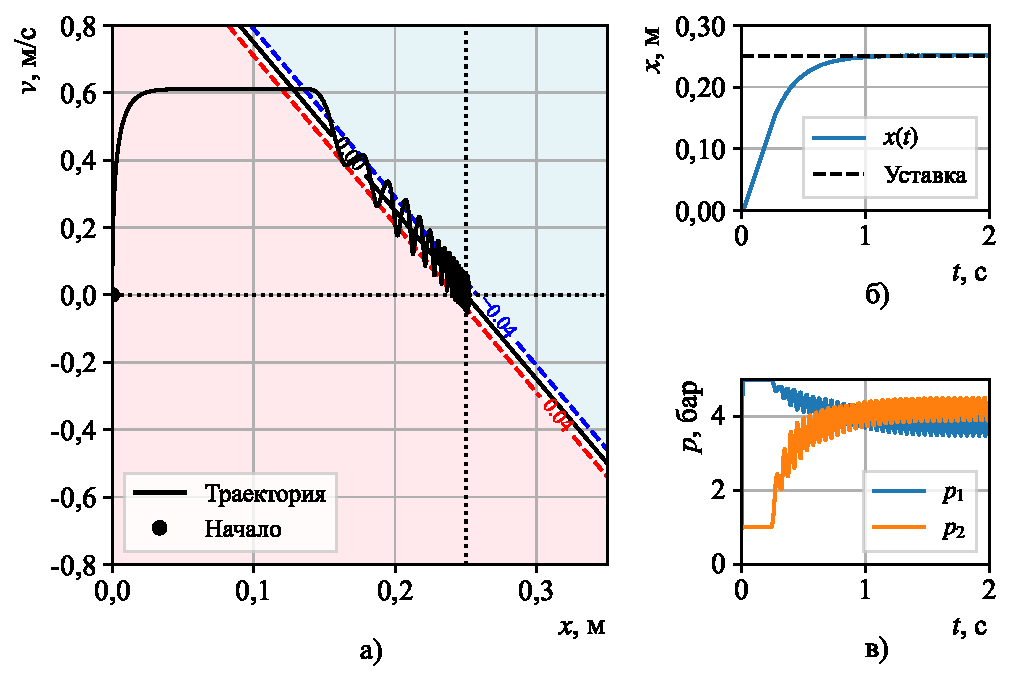
\includegraphics[]{part3/smc_linear_narrow.pdf}
	\caption{Динамика системы в скользящем режиме с линейной поверхностью первого порядка при $\lambda_1 = \num{5}$~и~$\varepsilon=\num{0.02}$: \\
		а) фазовый портрет; б) переходной процесс; в) изменение давлений в полостях}
	\label{fig:smc_linear_narrow}
\end{figure}

Интегральная поверхность скольжения задается уравнением:

\begin{equation}
	s_2 = \dot{e} + \lambda_1 e + \lambda_2 \int_0^t e(\tau)d\tau,
\end{equation}
где $\lambda_1$, $\lambda_2$ -- положительные коэффициенты.

Динамика ошибки описывается дифференциальным уравнением второго порядка:

\begin{equation}
	\ddot{e} + \lambda_1 \dot{e} + \lambda_2 e = 0.
\end{equation}

Характеристическое уравнение:

\begin{equation}
	p^2 + \lambda_1 p + \lambda_2 = 0,
\end{equation}
определяет характер переходного процесса. При $\lambda_1^2 > 4\lambda_2$ система демонстрирует
апериодический характер движения, при $\lambda_1^2 < 4\lambda_2$ -- колебательный.
Оптимальное соотношение $\lambda_1^2 = 4\lambda_2$ обеспечивает критический апериодический процесс.

Терминальная поверхность скольжения представляется выражением:

\begin{equation}
	s_3 = \dot{e} + \beta |e|^{q/p} \text{sign}(e),
\end{equation}

где $p$ и $q$ -- нечетные числа, удовлетворяющие условию $1 < q/p < 2$;
$\beta$ -- положительный коэффициент.

Динамика системы описывается нелинейным дифференциальным уравнением:
\begin{equation}
	\dot{e} = -\beta |e|^{q/p} \text{sign}(e).
\end{equation}

Особенность данной поверхности заключается в обеспечении конечного
времени сходимости, которое может быть вычислено аналитически:
\begin{equation}
	T_f = \frac{p}{\beta(p-q)}|e(0)|^{1-q/p}.
\end{equation}

Показатели степени $p$ и $q$ определяют характер
нелинейности: при $e \to 0$ скорость сходимости
увеличивается из-за того, что $q/p > 1$, что обеспечивает более быстрое достижение
целевого положения по сравнению с линейной поверхностью.

На рисунке \ref{fig:smc_terminal} представлены результаты моделирования для терминальной поверхности скольжения
при $p = 9$, $q = 11$ и $\beta = 5$.

\begin{figure}[ht]
	\centering
	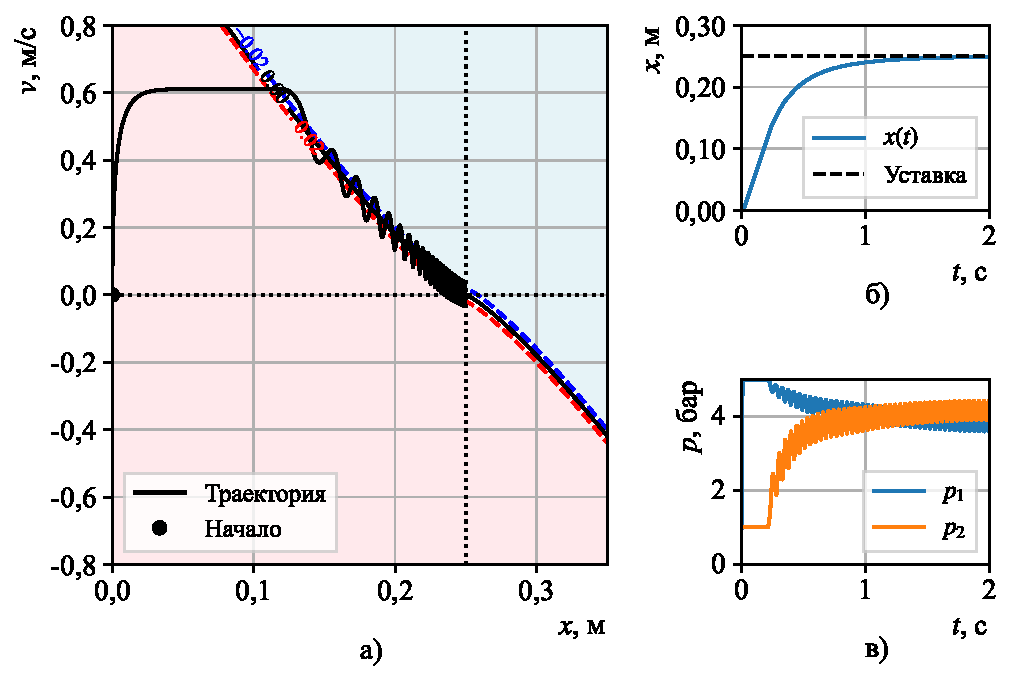
\includegraphics[]{part3/smc_teminal.pdf}
	\caption{Динамика системы в скользящем режиме с терминальной поверхностью скольжения при $p=9$, $q=11$ и $\beta=5$ \\
		а) фазовый портрет; б) переходной процесс; в) изменение давлений в полостях}
	\label{fig:smc_terminal}
\end{figure}


Для анализа устойчивости и качества движения вдоль каждой поверхности
скольжения рассмотрим соответствующие функции Ляпунова:
Для линейной поверхности скольжения функция Ляпунова имеет вид:
\begin{equation}
	V_1 = \frac{1}{2}s_1^2.
\end{equation}

Производная этой функции вдоль траекторий системы:
\begin{equation}
	\dot{V}_1 = s_1\dot{s}_1 = s_1(\ddot{e} + \lambda_1\dot{e}).
\end{equation}

При выполнении условия:

\begin{equation}
	s_1\dot{s}_1 \leq -\eta|s_1|
\end{equation}
где $\eta$ -- положительная константа, обеспечивается асимптотическая устойчивость скользящего режима.

Для интегральной поверхности расширенная функция Ляпунова учитывает интегральную составляющую:

\begin{equation}
	V_2 = \frac{1}{2}s_2^2 + \frac{\lambda_2}{2}\left(\int_0^t e(\tau)d\tau\right)^2.
\end{equation}
Её производная:

\begin{equation}
	\dot{V}_2 = s_2\dot{s}_2 + \lambda_2\left(\int_0^t e(\tau)d\tau\right)e.
\end{equation}

Условие существования устойчивого скользящего режима принимает вид:
\begin{equation}
	\dot{V}_2 \leq -\eta|s_2| - \gamma e^2.
\end{equation}
где $\gamma$ -- дополнительная положительная константа, обеспечивающая диссипацию энергии в интегральном канале.

Терминальная поверхность скольжения требует использования однородной функции Ляпунова:
\begin{equation}
	V_3 = \frac{1}{2}s_3^2 + \frac{\beta}{1+q/p}|e|^{1+q/p}.
\end{equation}

Производная этой функции:
\begin{equation}
	\dot{V}_3 = s_3\dot{s}_3 + \beta|e|^{q/p}\text{sign}(e)\dot{e}.
\end{equation}

Условие устойчивости:
\begin{equation}
	\dot{V}_3 \leq -\alpha_1|s_3| - \alpha_2|e|^{1+q/p},
\end{equation}
где $\alpha_1$, $\alpha_2$ -- положительные константы.

При многорежимном управлении переключение между режимами модифицирует
условия устойчивости. Для трехрежимного управления
область устойчивых движений определяется соотношением:
\begin{equation}
	\varepsilon < |s| < \beta_{\text{max}},
\end{equation}
где $\beta_{\text{max}}$ -- максимальное допустимое отклонение от поверхности скольжения.

При пятирежимном управлении возникают промежуточные зоны устойчивости:
\begin{equation}
	\begin{cases}
		\varepsilon_1 < |s| < \varepsilon_2      & \text{для промежуточных режимов} \\
		\varepsilon_2 < |s| < \beta_{\text{max}} & \text{для основных режимов}
	\end{cases}
\end{equation}

Семирежимное управление формирует наиболее сложную структуру областей устойчивости:
\begin{equation}
	\begin{cases}
		\varepsilon_1 < |s| < \varepsilon_2      & \text{для слабых режимов}  \\
		\varepsilon_2 < |s| < \varepsilon_3      & \text{для средних режимов} \\
		\varepsilon_3 < |s| < \beta_{\text{max}} & \text{для сильных режимов}
	\end{cases}
\end{equation}

Особый интерес представляет анализ поведения системы вблизи поверхности скольжения.
Для линейной поверхности скорость приближения к поверхности постоянна:
\begin{equation}
	\lim_{s_1 \to 0} \frac{\dot{s}_1}{s_1} = -\lambda_1.
\end{equation}

Для интегральной поверхности скорость приближения зависит от накопленной ошибки:
\begin{equation}
	\lim_{s_2 \to 0} \frac{\dot{s}_2}{s_2} = -\lambda_1 - \lambda_2\int_0^t e(\tau)d\tau.
\end{equation}

Терминальная поверхность обеспечивает переменную скорость приближения:
\begin{equation}
	\lim_{s_3 \to 0} \frac{\dot{s}_3}{s_3} = -\beta|e|^{q/p-1},
\end{equation}
что объясняет повышенное быстродействие при малых ошибках.